\subsection{Trajetórias betatron}
As equações \eqref{eq:2.20} e \eqref{eq:2.27} descrevem as oscilações betatron vertical e radial, respectivamente. Considerando as aproximações feitas, o movimento em cada coordenada é independente. Logo, como $K_x(s)$ e $K_z(s)$ tem a mesma forma matemática, toma-se a forma representativa
	
\begin{align}
	x'' = K(s) \; x \label{eq:2.31}
\end{align}
	
Lembrando que $K_x(s)$ descreve a oscilação betatron radial de um elétron com energia nominal $E_0$ e $K_z(s)$ descreve o movimento vertical.
	
A função de focalização $K(s)$ é definida em cada coordenada $s$ pelo design do anel de armazenamento. Se a posição e a inclinação ($x$ e $x'$) são dadas em alguma coordenada $s$, os termos subsequentes podem ser obtidos integrando a equação \eqref{eq:2.31}. Porém, como o campo guia é construído de segmentos magnéticos e $K(s)$ pode ser considerada constante nestes intervalos, pode-se integrar $x$ e $x'$ para cada segmento e juntar estes resultados. Dependendo do valor de $K$, $x$ é dado por

\begin{align}
	\left\{\begin{array}{l}
	K<0: \ \ x = a\ \cos(\sqrt{-K}s+b) \\
	K=0: \ \ x = as+b \\
	K>0: \ \ x = a\ \cosh(\sqrt{K}s+b)
	\end{array}\right. \label{eq:2.32}
\end{align}
onde $a$ e $b$ são constantes em cada segmento e podem ser determinadas pelos valores de $x$ e $x'$ na entrada do segmento (como $K$ é finita em qualquer ponto, $x$ e $x'$ devem ser ambas contínuas em todo ponto -- em particular, na junção entre dois segmentos).
	
\begin{proof}
	A equação \eqref{eq:2.31} é uma equação diferencial homogênea de 2ª ordem. Considerando que a função $K$ é uma constante, supõe-se que a solução da EDO é uma exponencial, 		ou seja, da forma $x=e^{rs}$. Substituindo esta possível solução, tem-se
	\begin{align*}
		x'' - Kx &=0\\
		(e^{rs})'' - K(e^{rs}) &= 0\\
		r^2e^{rs} - Ke^{rs}&=0\\
		(r^2 - K)e^{rs} &=0\\
		e^{rs} \neq 0 \therefore r^2 - K &= 0
	\end{align*}
	
	A equação $r^2 - K = 0$ é a equação característica da EDO. Resolvendo-a, tem-se $r = \pm \sqrt{K}$, então $x_{1,2} = e^{\pm\sqrt{K}s}$. Agora, existem 3 casos possíveis:
	\begin{itemize}
		\item $K<0$\\
			
		Com $K<0$, as raízes da equação característica são imaginárias. A solução geral da EDO é, para este caso, $x = c_1e^{\alpha s}\cos(\beta s) + c_2e^{\alpha s}\sin(\beta s)$. Como a função seno é apenas a função cosseno com uma diferença de fase, pode-se escrever
        \begin{align*}
        	x = a \ \cos(\sqrt{-K}+b)
        \end{align*}
			
		\item $K = 0$\\
		
		A solução geral da EDO é, para este caso, $x = c_1e^{\sqrt{K}s} + sc_2e^{-\sqrt{K}s}$. Como $K=0$, 
		\begin{align*}
            x &= c_1e^{\sqrt{K}s} + sc_2e^{-\sqrt{K}s}\\
            x &= c_1e^{0s} + sc_2e^{0s}\\
            x &= c_1 + sc_2
		\end{align*}
		
		Renomeando as constantes, $x = as + b$.

		\item $K > 0$\\
				
		A solução geral da EDO é, para este caso, $x = c_1e^{\sqrt{K}s} + c_2e^{-\sqrt{K}s}$. Fazendo $c_1=c_2=\frac{1}{2}$,
		\begin{align*}
            x &= c_1e^{\sqrt{K}s} + c_2e^{-\sqrt{K}s}\\
            x &= \frac{e^{\sqrt{K}s} + e^{-\sqrt{K}s}}{2} = cosh(\sqrt{K}x)
		\end{align*}
				
		Para constantes $c_1$ e $c_2$ arbitrárias,
		\begin{align*}
          x = a \ cosh(\sqrt{K}x + b)
		\end{align*}
	\end{itemize}
	
	Concluindo,
	\begin{align*}
        \left\{\begin{array}{l}
        K<0: \ \ x = a\ \cos(\sqrt{-K}s+b) \\
        K=0: \ \ x = as+b \\
        K>0: \ \ x = a\ \cosh(\sqrt{K}s+b)
        \end{array}\right.
	\end{align*}
\end{proof}

Como ilustração, supõe-se uma funçãoi $K(s)$ como a função $K_x(s)$ na \autoref{fig:fig10}. Duas possíveis trajetórias estão representadas na \autoref{fig:fig11} (b). A primeira é a trajetória que começa em $s_0$ com deslocamento unitário $x_0=1$ e nenhuma inclinação $x_0'=0$. A segunda começa com deslocamento nulo $x_0=0$ e inclinação unitária $x_0'= 1$. A primeira é chamada de \textit{cosinelike trajectory} -- $C$ e a segunda de \textit{sinelike trajectory} -- $S$. Seus detalhes dependem da coordenada de referência $s_0$ e são, em geral, funções não periódicas, mesmo que $K(s)$ seja. Para um anel com trajetórias estáveis, $C$ e $S$ são funções oscilatórias limitadas as quais possuem uma forma diferente a cada revolução.

\begin{figure}[!htb]
	\centering
	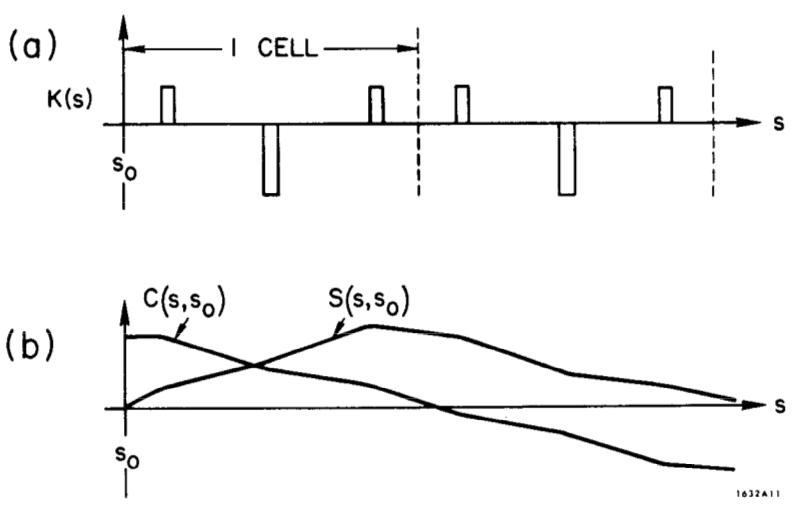
\includegraphics[width=0.7\linewidth]{./Figuras/fig11.jpeg}
	\caption{Função de focalização $K(s)$ e duas trajetórias: a \textit{cosine-like trajectory} e a \textit{sine-like trajectory} para uma coordenada de início $s_0 $. Retirado de \cite{sands1970physics}.}
	\label{fig:fig11}
\end{figure}
	
Agora, como a equação \eqref{eq:2.31} é linear em $x$, qualquer combinação linear de $C$ e $S$ também descreve uma trajetória possível para $x$. Mais que isso, qualquer trajetória pode ser descrita por esta combinação linear. Ou seja,
	
\begin{align}
	x(s) &= C(s,s_0)x_0 + S(s,s_0)x_0'\\
	x'(s) &= C'(s,s_0)x_0 + S'(s,s_0)x_0'
\end{align}
onde $C'$ e $S'$ são as derivadas de $C$ e $S$ em relação a $s$ e $x_0$ e $x_0'$ são os valores de $x$ e $x'$ em $s_0$. É conveniente escrever esta equação na forma matricial:
	
\begin{align}
	\boldsymbol{x}(s)=\boldsymbol{M}(s,s_0)\boldsymbol{x}(s_0)
\end{align}
onde 
\begin{align}
	\boldsymbol{x}(s) = \begin{bmatrix}
	x(s)\\ 
	x'(s)
	\end{bmatrix}
\end{align}
e
\begin{align}
	\boldsymbol{M}(s,s_0) = \begin{bmatrix}
	C(s,s_0) & S(s,s_0)\\
	C'(s,s_0) & S'(s,s_0)
	\end{bmatrix}\label{eq:2.37}
\end{align}
	
$\boldsymbol{M}(s,s_0)$ é a matriz de transferência de $s_0$ para $s$, a qual depende apenas de propriedades do campo guia entre duas coordenadas. A matriz de transferência de um trecho pode ser obtida em termos das matrizes de segmentos deste trecho. Logo, para um $s_1$ entre $s$ e $s_0$,
	
\begin{align}
	\boldsymbol{M}(s,s_0) = \boldsymbol{M}(s,s_1)\boldsymbol{M}(s_1,s_0)
\end{align}
	
\begin{proof}
	Pela definição da equação \eqref{eq:2.37},
	\begin{align*}
        \boldsymbol{M}(s,s_1) = \begin{bmatrix}
        C(s,s_1) & S(s,s_1)\\
        C'(s,s_1) & S'(s,s_1)
        \end{bmatrix}
	\end{align*} e
    \begin{align*}
		\boldsymbol{M}(s_1,s_0) = \begin{bmatrix}
		C(s_1,s_0) & S(s_1,s_0)\\
		C'(s_1,s_0) & S'(s_1,s_0)
		\end{bmatrix}
	\end{align*}
	
	Logo,
	\begin{align*}
        \boldsymbol{M}(s,s_0) &= \boldsymbol{M}(s,s_1)\boldsymbol{M}(s_1,s_0)\\
        &= \begin{bmatrix}
            C(s,s_1) & S(s,s_1)\\
            C'(s,s_1) & S'(s,s_1)
            \end{bmatrix} \begin{bmatrix}
                               C(s_1,s_0) & S(s_1,s_0)\\
                              C'(s_1,s_0) & S'(s_1,s_0)
                              \end{bmatrix}\\
        &= \begin{bmatrix}
        C(s,s_1)C(s_1,s_0)+S(s,s_1)C'(s_1,s_0) & C(s,s_1)S(s_1,s_0) + S(s,s_1)S'(s_1,s_0)\\
        C'(s,s_1)C(s_1,s_0)+S'(s,s_1)C'(s_1,s_0) & C'(s,s_1)S(s_1,s_0) + S'(s,s_1)S'(s_1,s_0)
        \end{bmatrix}	
	\end{align*}
	
	Considerando que $s_1 = s+\Delta_1$ e $s_0 = s_1 + \Delta_0$, então $(s,s_1) = \Delta_1$ e $(s_1,s_0) = \Delta_0$. Como $s_1$ é um ponto entre $s$ e $s_0$, também tem-se que $(s,s_0) = \Delta_1 + \Delta_0$. Logo, 
	\begin{align*}
        \boldsymbol{M}(\Delta_1)\boldsymbol{M}(\Delta_0) &= \begin{bmatrix}
        C(\Delta_1)C(\Delta_0)+S(\Delta_1)C'(\Delta_0) & C(\Delta_1)S(\Delta_0) + S(\Delta_1)S'(\Delta_0)\\
        C'(\Delta_1)C(\Delta_0)+S'(\Delta_1)C'(\Delta_0) & C'(\Delta_1)S(\Delta_0) + S'(\Delta_1)S'(\Delta_0)
        \end{bmatrix}
	\end{align*}
	
	Sabendo que $S'=C$ e $C'=-S$,
	\begin{align*}
        \boldsymbol{M}(\Delta_1)\boldsymbol{M}(\Delta_0) &= \begin{bmatrix}
        C(\Delta_1)C(\Delta_0)-S(\Delta_1)S(\Delta_0) & C(\Delta_1)S(\Delta_0) + S(\Delta_1)C(\Delta_0)\\
        -S(\Delta_1)C(\Delta_0)-C(\Delta_1)S(\Delta_0) & -S(\Delta_1)S(\Delta_0) + C(\Delta_1)C(\Delta_0)
        \end{bmatrix}
	\end{align*}
	
	Por propriedades trigonométricas,
	\begin{align*}
        [\boldsymbol{M}(\Delta_1)\boldsymbol{M}(\Delta_0)]_{11} &= \frac{1}{2}[C(\Delta_1-\Delta_0)+C(\Delta_1+\Delta_0)] - \frac{1}{2}[C(\Delta_1-\Delta_0)-C(\Delta_1+\Delta_0)]\\
        [\boldsymbol{M}(\Delta_1)\boldsymbol{M}(\Delta_0)]_{12} &= \frac{1}{2}[S(\Delta_1+\Delta_0)-S(\Delta_1-\Delta_0)] + \frac{1}{2}[S(\Delta_1-\Delta_0)+S(\Delta_1+\Delta_0)]\\
        [\boldsymbol{M}(\Delta_1)\boldsymbol{M}(\Delta_0)]_{21} &= -\frac{1}{2}[S(\Delta_1-\Delta_0)+S(\Delta_1+\Delta_0)] - \frac{1}{2}[S(\Delta_1+\Delta_0)-S(\Delta_1-\Delta_0)]\\
        [\boldsymbol{M}(\Delta_1)\boldsymbol{M}(\Delta_0)]_{22} &= -\frac{1}{2}[C(\Delta_1-\Delta_0)-C(\Delta_1+\Delta_0)] + \frac{1}{2}[C(\Delta_1-\Delta_0)+C(\Delta_1+\Delta_0)]
	\end{align*}
	
	Simplificando os termos da matriz, tem-se
	\begin{align*}
        \boldsymbol{M}(\Delta_1)\boldsymbol{M}(\Delta_0) &= \begin{bmatrix}
        C(\Delta_1+\Delta_0) & S(\Delta_1+\Delta_0)\\
        -S(\Delta_1+\Delta_0) & C(\Delta_1+\Delta_0)
        \end{bmatrix}\\
        &= \begin{bmatrix}
            C(\Delta_1+\Delta_0) & S(\Delta_1+\Delta_0)\\
            C'(\Delta_1+\Delta_0) & S'(\Delta_1+\Delta_0)
            \end{bmatrix}\\
        \boldsymbol{M}(s,s_1)\boldsymbol{M}(s_1,s_0)&= \begin{bmatrix}
            C(s,s_0) & S(s,s_0)\\
            C'(s,s_0) & S'(s,s_0)
            \end{bmatrix} = \boldsymbol{M}(s,s_0) 
	\end{align*}
	c.q.d.
\end{proof}
	
Para os três casos possíveis de $K$ descritos na equação \eqref{eq:2.32},
	
\begin{align}
	K<0: \ \ \boldsymbol{M}(s_2,s_1) &= \begin{bmatrix}
	\cos(\sqrt{-K}\ell) & \frac{1}{\sqrt{-K}}\sin(\sqrt{-K}\ell)\\
	-\sqrt{-K}\sin(\sqrt{-K}\ell) & \cos(\sqrt{-K}\ell)
	\end{bmatrix}\\
	K=0: \ \ \boldsymbol{M}(s_2,s_1) &= \begin{bmatrix}
		1 & \ell\\
		0 & 1
		\end{bmatrix}\\
	K>0: \ \ \boldsymbol{M}(s_2,s_1) &= \begin{bmatrix}
		\cosh(\sqrt{K}\ell) & \frac{1}{\sqrt{K}}\sinh(\sqrt{K}\ell)\\
		\sqrt{K}\sinh(\sqrt{K}\ell) & \cosh(\sqrt{K}\ell)
		\end{bmatrix}
\end{align}
onde $\ell = s_2-s_1$.
	
\begin{proof}Analisando para os três casos de $K$:
	\begin{itemize}
	\item $K<0$\\
	
	Da equação \eqref{eq:2.32}, tem-se que $C(s_2,s_1) = \cos(\sqrt{-K}\ell)$. Logo,
	\begin{align*}
        C'(s_2,s_1) &= \frac{d\ \cos(\sqrt{-K}\ell)}{d\ell} = -\sqrt{-K}\sin(\sqrt{-K}\ell)\\
        S(s_2,s_1) &= \int \cos(\sqrt{-K}\ell)d\ell = \frac{1}{\sqrt{-K}}\sin(\sqrt{-K}\ell)\\
        \therefore \boldsymbol{M}(s_2,s_1) &= \begin{bmatrix}
            \cos(\sqrt{-K}\ell) & \frac{1}{\sqrt{-K}}\sin(\sqrt{-K}\ell)\\
            -\sqrt{-K}\sin(\sqrt{-K}\ell) & \cos(\sqrt{-K}\ell)
            \end{bmatrix}
	\end{align*}
	\item $K=0$\\
	
	Da equação \eqref{eq:2.32}, tem-se que $C(s_2,s_1) = 1$. Logo,
	\begin{align*}
		C'(s_2,s_1) &= \frac{d \ 1}{d\ell} = 0\\
		S(s_2,s_1) &= \int d\ell = \ell\\
		\therefore \boldsymbol{M}(s_2,s_1) &= \begin{bmatrix}
				1 & \ell\\
				0 & 1
				\end{bmatrix}
	\end{align*}
	\item $K>0$\\
	
	Da equação \eqref{eq:2.32}, tem-se que $C(s_2,s_1) = \cosh(\sqrt{K}\ell)$. Logo,
		\begin{align*}
        	C'(s_2,s_1) &= \frac{d\ \cosh(\sqrt{K}\ell)}{d\ell} = \sqrt{K}senh(\sqrt{K}\ell)\\
            S(s_2,s_1) &= \int \cosh(\sqrt{K}\ell)d\ell = \frac{1}{\sqrt{K}}senh(\sqrt{K}\ell)\\
            \therefore \boldsymbol{M}(s_2,s_1) &= \begin{bmatrix}
            \cosh(\sqrt{K}\ell) & \frac{1}{\sqrt{K}}\sinh(\sqrt{K}\ell)\\
            \sqrt{K}\sinh(\sqrt{K}\ell) & \cosh(\sqrt{K}\ell)
            \end{bmatrix}
		\end{align*}
	\end{itemize}
\end{proof}
	
A solução geral da equação \eqref{eq:2.31} pode ser escrita como
	
\begin{align}
	x(s) = a\zeta(s)\ cos\{\varphi(s)-\upsilon\}\label{eq:2.39}
\end{align}
onde $\zeta(s)$ e $\varphi(s)$ são funções especialmente definidas em $s$ com certas propriedades convenientes, e $a$ e $\upsilon$ são constantes obtidas pelas condições iniciais, as quais determinam uma trajetória particular. Define-se
	
\begin{align}
	\varphi(s) = \int_{0}^{s} \frac{d\bar{s}}{\zeta^2(\bar{s})}
\end{align}
	
Então
\begin{align}
	\varphi'(s) = \frac{1}{\zeta^2}
\end{align}
e, se $\zeta(s)$ for definida para ser essa função positiva, analítica que satisfaz
\begin{align}
	\zeta'' = K(s)\zeta+\frac{1}{\zeta^3}\label{eq:2.41}
\end{align}
então $x(s)$ da equação \eqref{eq:2.39} satisfaz a equação diferencial \eqref{eq:2.31}.
	
\begin{proof}
	Seja $x(s)$ dado pela equação \eqref{eq:2.39}. Então,
	\begin{align*}
        x' &= [a\zeta\ \cos\{\varphi-\upsilon\}]'\\
        &= a[\zeta'\cos(\varphi-\upsilon)-\zeta\varphi'\sin(\varphi-\upsilon)]\\
        \therefore x'' &= a[\zeta'\cos(\varphi-\upsilon)-\zeta\varphi'\sin(\varphi-\upsilon)]'\\
        &= a\left[\zeta''\cos(\varphi-\upsilon)-\zeta'\varphi'\sin(\varphi-\upsilon) - \left(-\frac{\zeta'}{\zeta^2}\sin(\varphi-\upsilon)+\frac{\varphi'}{\zeta}\cos(\varphi-\upsilon)\right)\right]
	\end{align*}
	
	Pela equação \eqref{eq:2.41}, 
	\begin{align*}
        x'' &= a\left[\left(K\zeta+\frac{1}{\zeta^3}\right)\cos(\varphi-\upsilon)-\frac{\zeta'}{\zeta^2}\sin(\varphi-\upsilon) + \frac{\zeta'}{\zeta^2}\sin(\varphi-\upsilon)-\frac{1}{\zeta^3}\cos(\varphi-\upsilon)\right]\\
        &= Ka\zeta\ \cos(\varphi-\upsilon)\\
        &= Kx
	\end{align*}
	
	Assim, pode-se ver que $x(s) = a\zeta(s)\ \cos\{\varphi(s)-\upsilon\}$ é solução da equação diferencial \eqref{eq:2.31}.
\end{proof}
	
Tradicionalmente, define-se a função betatron $\beta(s)$ como
\begin{align}
	\beta(s) = \zeta^2(s)
\end{align}
então
\begin{align}
	x(s) &= a\sqrt{\beta(s)}\ \cos\{\varphi(s)-\upsilon\}\label{eq:2.43}\\
	\varphi(s) &= \int_{0}^{s} \frac{d\bar{s}}{\beta(\bar{s})}\label{eq:2.44}
\end{align}
	
Note que, dada a função de focalização $K(s)$ do anel, $\beta(s)$ pode ser unicamente determinada. Porém, enquanto $K(s)$ é dada em função das propriedades locais do campo guia, a função $\beta(s)$ -- ou $\zeta(s)$ depende da configuração total do anel. Por outro lado, uma vez que $\beta(s)$ é conhecida, $K(s)$ pode ser imediatamente determinada pelas suas derivadas locais, mas é $\beta(s)$ que revela de forma mais direta as características significantes da trajetória dos elétrons armazenados.
	
Lembrando que toda a discussão feita nesta subsseção se aplica tanto no movimento radial quanto no vertical, ou seja, o anel é descrito pelas funções $\beta_x$ e $\beta_z$, as quais são derivadas das funções de focalização $K_x$ e $K_z$, respectivamente.